\documentclass{article}
\usepackage[utf8]{inputenc}
\usepackage{geometry}
\geometry{
	paperwidth=35cm,
	paperheight=48cm,
	% textwidth=35cm,
	% textheight=48cm,
	% total={35cm,48cm},
	top=3cm,
	bottom=2cm,
	left=2cm,
	right=2cm,
}
\usepackage{graphicx}
\graphicspath{{../plots/}}
\usepackage{subcaption}
\usepackage[font=large,labelfont=bf]{caption}
\captionsetup{width=\textwidth}


\begin{document}

	\begin{figure} [h!]
		\centering
		\begin{subfigure} {\columnwidth}
				\centering 
				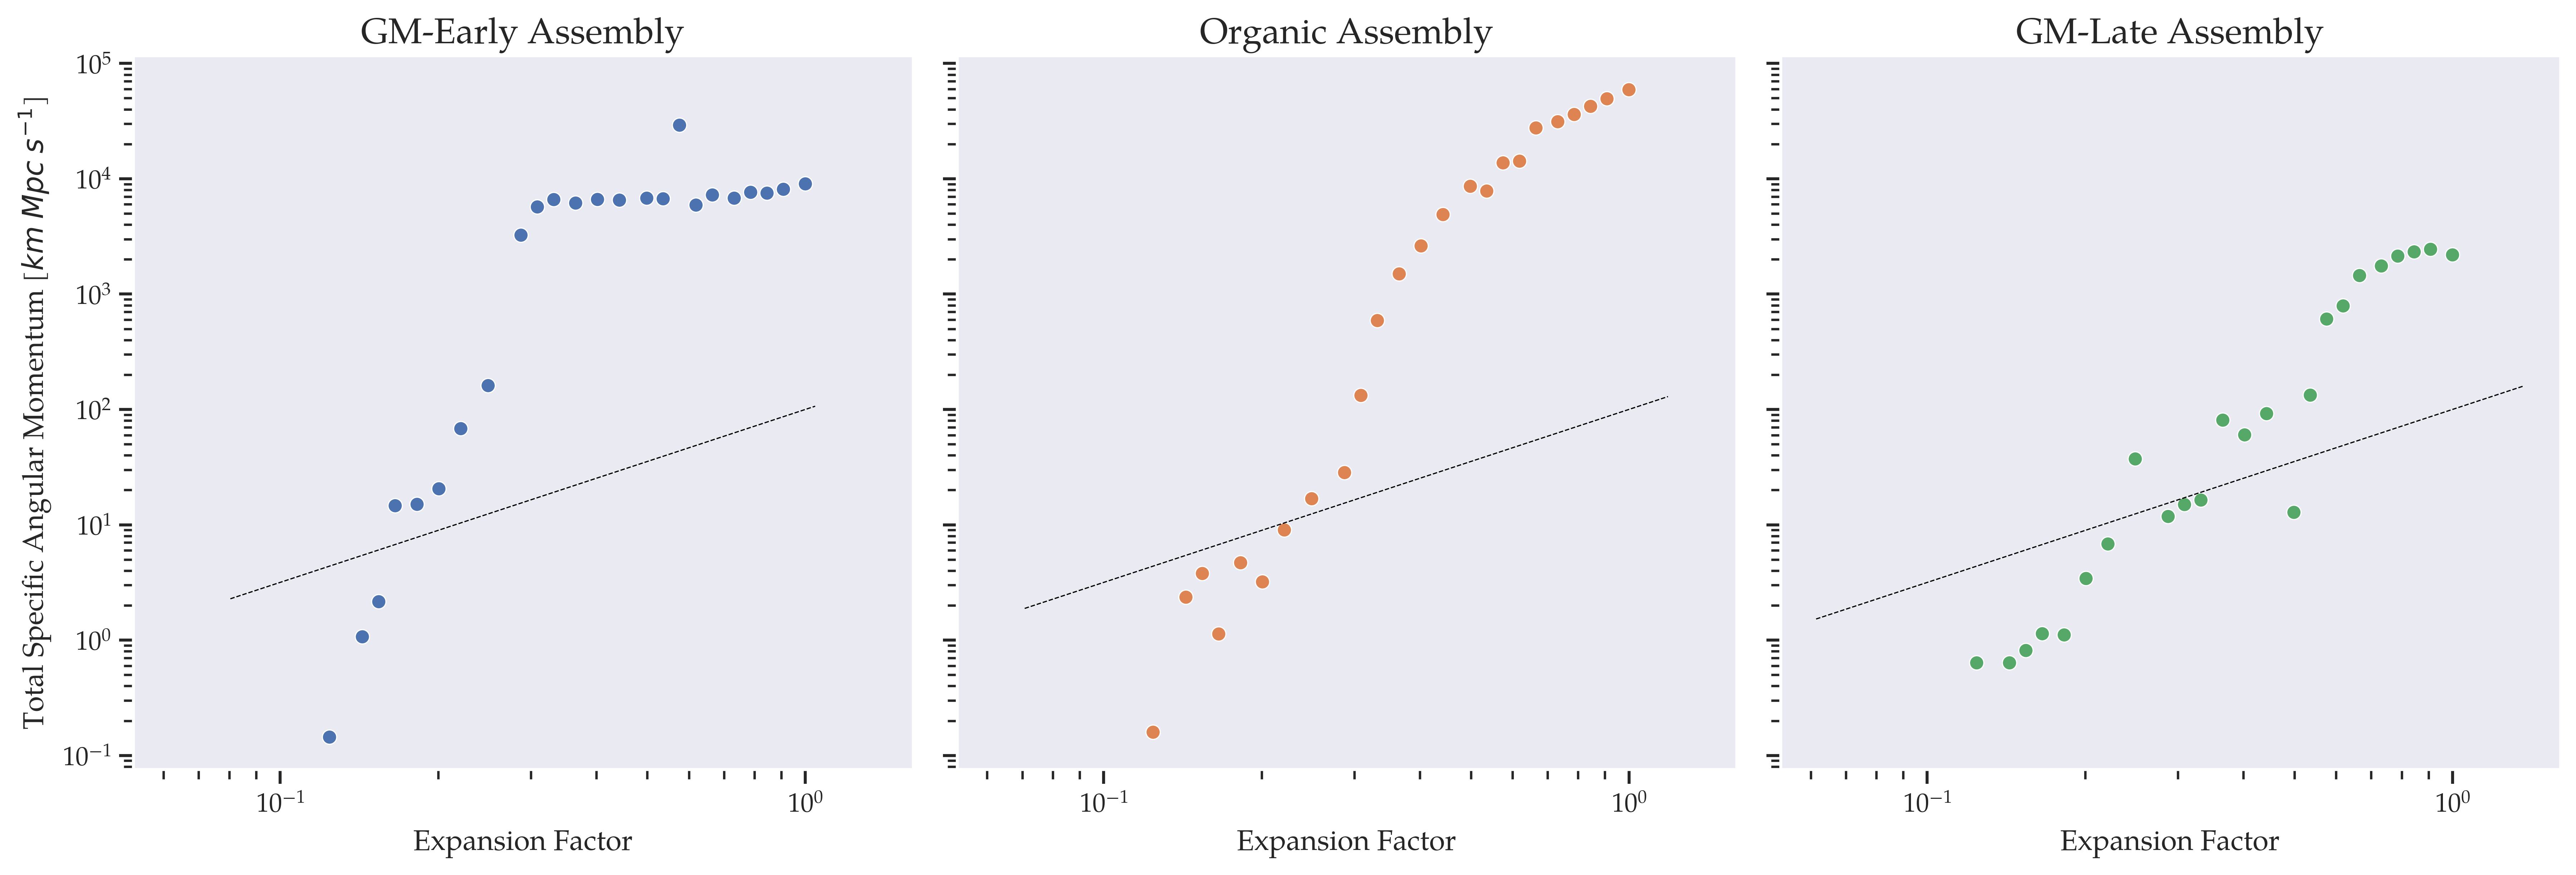
\includegraphics[width=\columnwidth]{../../plots/baryon_cdm/expansion_factor-net_specific_angular_momentum.png}
				\caption{Total specific angular momentum vs expansion factor plot for three assembly modes.}
		\end{subfigure} \\
			% \hfill
			\vspace{1cm}
		\begin{subfigure} {\columnwidth}
				\centering 
				\includegraphics[width=\columnwidth]{../../plots/baryon_cdm/expansion_factor-net_specific_angular_momentum_baryons.png}
				\caption{Total specific angular momentum vs expansion factor plot for \emph{baryon }particles in three assembly modes.}
		\end{subfigure} \\
			\vspace{1cm}
		\begin{subfigure} {\columnwidth}
				\centering 
				\includegraphics[width=\columnwidth]{../../plots/baryon_cdm/expansion_factor-net_specific_angular_momentum_cdm.png}
				\caption{Total specific angular momentum vs expansion factor plot for \emph{cold dark matter} particles in three assembly modes.}
		\end{subfigure}
		\caption{Specific angular momentum vs expansion factor (\(a\)) plots, overlaid by \(a^{3/2}\) dashed black line.}
	\end{figure} 

	\Large 
	\begin{itemize}
		\item The bottom two subplots (for baryons and CDM, respectively) add up to give the uppermost subplot (baryons and CDM combined).
		\item As speculated earlier last week, at lower redshifts, \(L_{specific}\) is rising to higher values in GM-Late case than in Organic case.
		\item Overall trends seem roughly consistent with the \(a^{3/2}\) law.
		\item The evolution is not as smooth as that obtained for inner 30kpc data, especially for GM-Late data at lower redshifts.
		\item To compare figure 3 Zavala et al. (2016), there are discrepancies, especially in disc-dominated -- GM-Late case. Total specific angular momentum does not seem to decline at lower redshifts.
		\item When compared to figures 6 and 3-left from Zavala et al. (2008), the trends look somewhat fine, especially for the dark matter halo.  
	\end{itemize} 

	\clearpage

	\begin{figure} [h!]
		\centering
		\begin{subfigure} {\columnwidth}
				\centering 
				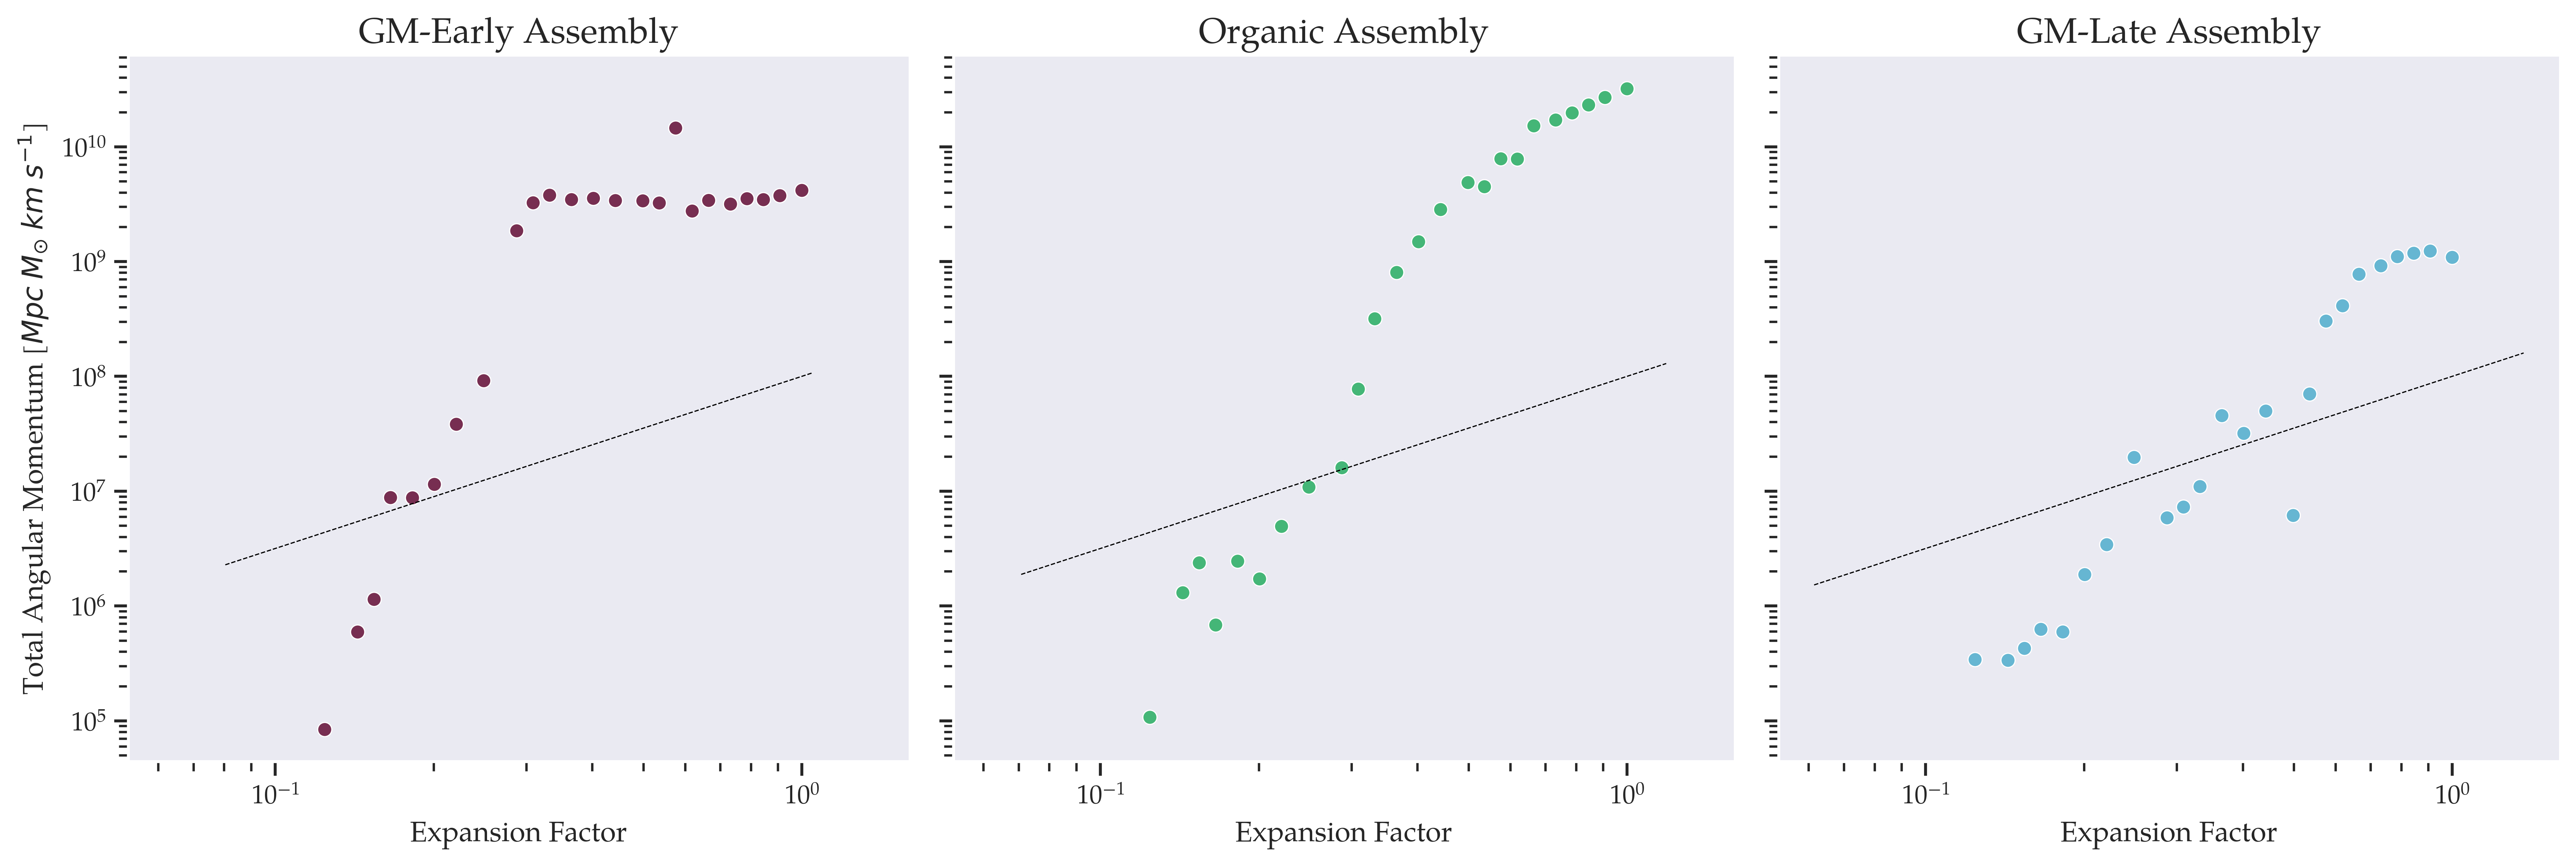
\includegraphics[width=\columnwidth]{../../plots/baryon_cdm/expansion_factor-net_angular_momentum.png}
				\caption{Total angular momentum vs expansion factor plot for three assembly modes.}
		\end{subfigure} \\
			% \hfill
			\vspace{1cm}
		\begin{subfigure} {\columnwidth}
				\centering 
				\includegraphics[width=\columnwidth]{../../plots/baryon_cdm/expansion_factor-net_angular_momentum_baryons.png}
				\caption{Total angular momentum vs expansion factor plot for \emph{baryon }particles in three assembly modes.}
		\end{subfigure} \\
			\vspace{1cm}
		\begin{subfigure} {\columnwidth}
				\centering 
				\includegraphics[width=\columnwidth]{../../plots/baryon_cdm/expansion_factor-net_angular_momentum_cdm.png}
				\caption{Total angular momentum vs expansion factor plot for \emph{cold dark matter} particles in three assembly modes.}
		\end{subfigure}
		\caption{Total angular momentum vs expansion factor (\(a\)) plots, overlaid by \(a^{3/2}\) dashed black line.}
	\end{figure}

	\Large 
	\begin{itemize}
		\item Final mass of baryons is of the order of \(10^{11}\). So, angular momentum and specific angular momentum values seem roughly consistent.
		\item With dark matter halo mass of the order of \(10^{-32}\), values of total angular momentum of cold dark matter also seems fine.
		\item It might be of interest that the total angular momentum is still increasing faster than \(a^{3/2}\). (Although I am not sure, this rise seems slightly gradual when compared to last week's plots.)
	\end{itemize} 

	\clearpage 

	\begin{figure} [h!]
		\centering
		\begin{subfigure} {\columnwidth}
				\centering 
				\includegraphics[width=\columnwidth]{../../plots/baryon_cdm/expansion_factor-net_specific_angular_momentum_a3by2.png}
				\caption{Total specific angular momentum divided by expansion factor raised to the 3/2 exponent vs expansion factor plot for three assembly modes.}
		\end{subfigure} \\
			% \hfill
			\vspace{1cm}
		\begin{subfigure} {\columnwidth}
				\centering 
				\includegraphics[width=\columnwidth]{../../plots/baryon_cdm/expansion_factor-net_specific_angular_momentum_a3by2_baryons.png}
				\caption{Total specific angular momentum divided by expansion factor raised to the 3/2 exponent vs expansion factor plot for \emph{baryon} particles in three assembly modes.}
		\end{subfigure} \\
			\vspace{1cm}
		\begin{subfigure} {\columnwidth}
				\centering 
				\includegraphics[width=\columnwidth]{../../plots/baryon_cdm/expansion_factor-net_specific_angular_momentum_a3by2_cdm.png}
				\caption{Total specific angular momentum divided by expansion factor raised to the 3/2 exponent vs expansion factor plot for \emph{cold dark matter} particles in three assembly modes.}
		\end{subfigure}
		\caption{Specific angular momentum divided by expansion factor raised to the 3/2 exponent vs expansion factor (\(a\)) plots, overlaid by \(a^{3/2}\) dashed black line.}
	\end{figure}

	\begin{itemize}
		\item I just hope I plotted these correctly because these don't really look fine to me. 
		\item Divided the y axes values with \(a^{3/2}\) in order to compare with figures 3 and 5 of Zavala et al. (2008).
	\end{itemize}

	\clearpage 
	\begin{figure} 
		\centering 
		\includegraphics[width=\columnwidth]{../../plots/baryon_cdm/expansion_factor-net_specific_angular_momentum_combined_only_L.png}
		\caption{Specific angular momentum variation for baryonic and cold dark matter as a function of expansion factor for three assembly modes.}
	\end{figure}

\end{document}